\documentclass[a4paper,landscape]{article}
\def\micro{\mu m}
\def\um{$\micro$ }
\def\degreesC{$\degree$C }
\def\percent{$\%$ }
\def\rowHeight{35pt}

\usepackage{geometry}
\geometry{
%	a4paper,
%	total={170mm,257mm},
	a3paper,
	left=5mm,
	top=5mm,
	right=5mm,
	bottom=15mm,
}

\usepackage[dvipsnames]{xcolor}

%%  -------------------------------------------------------------------
%%      GDS II layer, regarding MOSIS SCMOS layer map
%%  -------------------------------------------------------------------
% GDS II #41 - P_WELL
\definecolor{pwell}{rgb}{1.0, 0.74, 0.53}   % macaroni and cheese
% GDS II #42 - N_WELL
\definecolor{nwell}{rgb}{0.61, 0.87, 1.0}  % columbia blue
\definecolor{pbase}{rgb}{1.0, 0.51, 0.26}  % mango tango
\definecolor{nbase}{rgb}{0.0, 0.75, 1.0}   % capri 
% GDS II #43 - ACITVE
\definecolor{active}{rgb}{0.9, 0.4, 0.38}   % light carmine pink
% GDS II #45 - N_PLUS_SELECT
\definecolor{nimplant}{rgb}{0.45, 0.76, 0.983}% maya blue
% GDS II #44 - P_PLUS_SELECT
\definecolor{pimplant}{rgb}{1.0, 0.51, 0.26}% mango tango
% GDS II #46 - POLY
\definecolor{poly}{rgb}{0.56, 0.93, 0.56}   % light green
% GDS II #25 - CONTACT
\definecolor{contact}{rgb}{0.83, 0.83, 0.83}% light gray
% GDS II #49 - METAL1
\definecolor{metal1}{rgb}{0.38, 0.31, 0.86} % majorelle blue
% GDS II #50 - VIA1
\definecolor{via1}{rgb}{0.83, 0.83, 0.83}   % light gray
% GDS II #51 - METAL2
\definecolor{metal2}{rgb}{0.04, 0.85, 0.32} % malachite
% GDS II #61 - VIA2
\definecolor{via2}{rgb}{0.83, 0.83, 0.83}   % light gray
% GDS II #63 - METAL3
\definecolor{metal3}{rgb}{0.98, 0.93, 0.37} % maize
% GDS II #30 - VIA3
\definecolor{via3}{rgb}{0.83, 0.83, 0.83}   % light gray
% GDS II #31 - METAL4
\definecolor{metal4}{rgb}{0.75, 0.25, 0.0}  % mahogany
% GDS II #32 - VIA4
\definecolor{via4}{rgb}{0.83, 0.83, 0.83}   % light gray
% GDS II #33 - METAL5
\definecolor{metal5}{rgb}{0.79, 0.08, 0.48} % magenta (dye)
% GDS II #36 - VIA5
\definecolor{via5}{rgb}{0.83, 0.83, 0.83}   % light gray
% GDS II #37 - METAL6
\definecolor{metal6}{rgb}{0.11, 0.35, 0.02} % lincoln green
% GDS II #29 - SILICIDE_BLOCK
\definecolor{silicide-block}{rgb}{0.98, 0.94, 0.9}  % linen
% GDS II #52 - GLASS
\definecolor{glass}{rgb}{1.0, 1.0, 0.88}    % light yellow
% GDS II #26 - PADS
\definecolor{pads}{rgb}{0.75, 1.0, 0.0}     % lime (color wheel)

\definecolor{resist}{rgb}{0.71, 0.4, 0.11}  % light brown

\definecolor{silicide}{rgb}{0.29, 0.33, 0.13}
\definecolor{titanium}{rgb}{0.8, 0.58, 0.46}

\def\OpacityLayout {0.5}

%
% physical
%
\definecolor{substrate}{rgb}{0.96, 0.94, 0.93}  % isabelline
\definecolor{nitride}{rgb}{1.0, 0.03, 0.0}
\definecolor{gateoxide}{rgb}{0.88, 1.0, 1.0}    % light cyan
\definecolor{isolationoxide}{rgb}{0.84, 0.79, 0.87}% languid lavender

\usepackage[utf8]{inputenc}
\usepackage[english]{babel}
\usepackage{forloop}
\usepackage{array}
\usepackage{amsmath}
\usepackage{amsfonts}
\usepackage{amssymb}
\usepackage{gensymb}
\usepackage{mdframed}
\usepackage{graphicx}
\usepackage{tikz}

\usetikzlibrary{
	arrows,
	automata,
        shadings,
        shadows,
        shapes,
}
\usepackage[siunitx]{circuitikz}
\usepackage{makecell}
\usepackage{array}

\usepackage[colorlinks=true,linkcolor=blue,urlcolor=black,bookmarksopen=true]{hyperref}
\usepackage{bookmark}
\usepackage{hyperref}
\usepackage{sepfootnotes}
\usepackage{lipsum,tocloft} 
\usetikzlibrary{positioning}
\usetikzlibrary{patterns}

\newlength{\struthd}
\newcommand*\Strut[2][-0.3]{%
	\setlength{\struthd}{#2}%
	\rule[#1\struthd]{0pt}{\struthd}%
}

\usepackage{float}
\floatstyle{boxed} 
\restylefloat{figure}

\newcolumntype{C}[1]{>{\centering\arraybackslash}m{#1}} % zentriert mit Breitenangabe

\def\CrossSectionOnly{0.3}
\def\CrossAndTopSection{0.2}
\def\CrossAndTopSectionBig{0.3}
\def\VLSILayout{0.4}
\def\UpperContactResist{8.0}
\def\UpperMetalResist{9.0}
\def\UpperMoreMetalResist{16.0}

\def\LowerMetal{4.0}
\def\UpperMetal{4.5}

\def\LowerMoreMetal{5.0}
\def\UpperMoreMetal{5.5}

\def\LowerMoreMetalTwo{6.0}
\def\UpperMoreMetalTwo{6.5}

\def\UpperGlass{7.0}


\newcounter{TopProcessStep}
\newcounter{SubProcessStep}
\setcounter{TopProcessStep}{0}
\setcounter{SubProcessStep}{1}

\def\LastCleaniness{foo}

\newcommand{\getWaferCleaninessSymbol}[1]{
	\ifthenelse{\equal{#1}{clean}}{
\begin{tikzpicture}\node [fill=cyan, rounded corners=5pt] {Clean};\end{tikzpicture}} {
		\ifthenelse{\equal{#1}{semi-clean}} {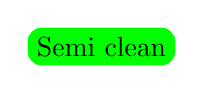
\begin{tikzpicture}\node [fill=green, rounded corners=5pt] {Semi clean};\end{tikzpicture}} {
			\ifthenelse{\equal{#1}{clean/semi-clean}} {
				
\begin{tikzpicture}
					\node [fill=cyan, rounded corners=5pt] at (0,0.0) {Clean};
					\node [fill=green, rounded corners=5pt] at (1.5,0.0) {Semi clean};
				\end{tikzpicture}
			} {
				\ifthenelse{\equal{#1}{non-standard}} {
					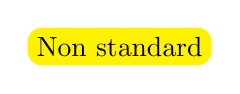
\begin{tikzpicture}
						\node [fill=yellow, rounded corners=5pt] {Non standard};
					\end{tikzpicture}} {undef}
			}
		}
	}
}

\newcommand{\makeProcessTable}[5]{
	\setcounter{SubProcessStep}{0}
	\addtocounter{TopProcessStep}{1}
	\newpage
	\section{#1}
	\begin{center}
	\fbox{\begin{minipage}{\textwidth}
		\centering
		\begin{tikzpicture}[node distance = 3cm, auto, thick, scale=0.7, every node/.style={transform shape}]
			\input{#2}
		\end{tikzpicture}\\
		\textbf{Mask: #3}
	\end{minipage}}

	\begin{tabular}{|>{\Strut[-0.5]{\rowHeight}}r|}
		\hline
		\textbf{Wafer Cleanliness} \\
		#4
		\hline
        \end{tabular}
	\hspace{0.25cm}
        \begin{tabular}{
			|>{\Strut[-0.5]{\rowHeight}}r
			|C{8.0cm}
			|C{2.0cm}
			|C{3.0cm}
			|C{5.0cm}
			|C{9.0cm}
			|}
		\hline
		\textbf{Step Number} &
		\textbf{Equipment} &
		\textbf{Location} &
		\textbf{Cleanliness} &
		\textbf{Process} &
		\textbf{Requirements} \\
		#5
		\hline
	\end{tabular}
	\end{center}
}

\newcommand{\addProcessStep}[5]{
	\hline
	\addtocounter{SubProcessStep}{1}
	\arabic{TopProcessStep}.\arabic{SubProcessStep} &
	#1 &
	#2 &
	\getWaferCleaninessSymbol{#3} &
	#4 &
	#5
	%\\[0.5cm]
	\\
}

\newcommand{\addLevelCell}[1]{
	\hline
	\getWaferCleaninessSymbol{#1}
	%\\[0.5cm]
	\\
}

\author{David Lanzendörfer}
\title{LibreSilicon process HKUST (NFF)}
\begin{document}
\maketitle
\begin{abstract}
	Copyright © 2017 LANCEVILLE TECHNOLOGY GROUP CO., LIMITED. All rights reserved. \\

This process is licensed under the Libre Silicon public license; you can redistribute it and/or modify it under the terms of the Libre Silicon public license
as published by the Libre Silicon alliance, either version 1 of the License, or (at your option) any later version.

This design is distributed in the hope that it will be useful, but WITHOUT ANY WARRANTY; without even the implied warranty of MERCHANTABILITY or FITNESS FOR A PARTICULAR PURPOSE.
See the Libre Silicon Public License for more details. \\

This document is part of the specification of the free silicon manufacturing standard for manufacturing the LibreSilicon standard logic cells\footnote{\url{https://github.com/chipforge/StdCellLib}} and related free technology nodes from the LibreSilicon project.

For this initial revision 0.1 a gate-first approach has been chosen which led to the choice of polysilicon as the gate electrode material because of the simplicity of the gate alignment.
For better isolation properties of the transistors and gates in overall a box-isolation approach has been chosen.
All of these choices have been made with the future scale down from the recent $1 \mu m$ to smaller structure sizes.
\textbf{This process is for manufacturing $1 \mu m$ only!}
But further releases which will have been tested with smaller structure sizes can be expected.
 \\
	Please see the document with the generic steps\footnote{\url{https://github.com/libresilicon/process/raw/master/process_steps/process_hightech/process_hightech_steps.pdf}}
	in order to get a detailed description of the different steps.	
\end{abstract}
\vfill
\newpage

Process Flow of Lanceville Technologies LibreSilicon 1\um 

\begin{itemize}
	\item Project: LibreSilicon 1\um
	\item Name: Lanceville Technologies Group
	\item Substrate: P-Substrate silicon wafer <100>
	\item Date: \today
\end{itemize}

\begin{mdframed}[linewidth=2pt,linecolor=black]
\begin{center}
	\begin{tikzpicture}[node distance = 3cm, auto, thick,scale=0.5, every node/.style={transform shape}]
		\fill[isolationoxide] (0,\LowerMoreMetalTwo) rectangle (20,\UpperMoreMetalTwo);

\fill[isolationoxide] (0,\UpperMoreMetalTwo) rectangle (2.75,\UpperGlass);
\fill[isolationoxide] (8.25,\UpperMoreMetalTwo) rectangle (11.75,\UpperGlass);
\fill[isolationoxide] (17.25,\UpperMoreMetalTwo) rectangle (20,\UpperGlass);

\fill[metal3] (3.5,\LowerMoreMetal) rectangle (7.5,\LowerMoreMetalTwo);
\fill[metal3] (12.5,\LowerMoreMetal) rectangle (16.5,\LowerMoreMetalTwo);

\fill[metal3] (2,\LowerMoreMetalTwo) rectangle (9,\UpperMoreMetalTwo);
\fill[metal3] (11,\LowerMoreMetalTwo) rectangle (18,\UpperMoreMetalTwo);

\fill[isolationoxide] (0,\LowerMoreMetal) rectangle (3.5,\LowerMoreMetalTwo);
\fill[isolationoxide] (7.5,\LowerMoreMetal) rectangle (12.5,\LowerMoreMetalTwo);
\fill[isolationoxide] (16.5,\LowerMoreMetal) rectangle (20.0,\LowerMoreMetalTwo);

\input{tikz_process_steps/more_metal.a.tex}



	\end{tikzpicture}
\end{center}
\end{mdframed}
\newpage

\makeProcessTable{Initial alignment mask}{tikz_process_steps/basic.a.tex}{basic}{\addLevelCell{clean} %Default cleaning
\addLevelCell{clean} %Dry the wafer automatically
\addLevelCell{clean} %HMDS, PR coating, soft bake
\addLevelCell{clean} %Exposure of the layer
\addLevelCell{clean} %Develop, Hard bake
\addLevelCell{clean} %Etching the alignment crosses from HKUST
\addLevelCell{clean} %Resist strip
\addLevelCell{clean} %Resist strip
\addLevelCell{clean} %Dry the wafer automatically
}{\addProcessStep{B1: Sulfuric cleaning (WET-B1)}{P2-01000}{clean}{Default cleaning}{}
\addProcessStep{Spin Dryer-B (SRD-B)}{P2-01000}{clean}{Dry the wafer automatically}{}
\addProcessStep{SVG Coater Track (PHT-T1)}{P2-00100}{clean/semi-clean}{HMDS, PR coating, soft bake}{HPR 504: 3krpm ( $\approx$1.5\um ), soft bake: 110\degreesC 1min}
\addProcessStep{ASML Stepper (PHT-S1)}{P2-00100}{clean/semi-clean}{Exposure of the layer}{}
\addProcessStep{SVG Developer Track (PHT-T2)}{P2-00100}{clean/semi-clean}{Develop, Hard bake}{FHD-5, 1min; hard bake: 120\degreesC, 1min}
\addProcessStep{Lam 490 etcher (DRY-490)}{P2-01000}{clean}{Etching the alignment crosses from HKUST}{2 minutes (120nm)}
\addProcessStep{PS210 Asher (DRY-PR-1)}{P2-01000}{clean}{Resist strip}{}
\addProcessStep{E4:Resist strip (WET-E4)}{P2-01000}{clean/semi-clean}{Resist strip}{}
\addProcessStep{Spin Dryer-E (SRD-E)}{P2-01000}{clean/semi-clean}{Dry the wafer automatically}{}
}
\makeProcessTable{P-well}{tikz_process_steps/pwell.a.tex}{pwell}{\addLevelCell{clean} %Default cleaning
\addLevelCell{clean} %Dry the wafer automatically
\addLevelCell{clean} %HMDS, PR coating, soft bake
\addLevelCell{clean} %Exposure of the layer
\addLevelCell{clean} %Develop, Hard bake
\addLevelCell{clean} %Boron implant
\addLevelCell{clean} %Resist strip
\addLevelCell{clean} %Resist strip
\addLevelCell{clean} %Dry the wafer automatically
}{\addProcessStep{B1: Sulfuric cleaning (WET-B1)}{P2-01000}{clean}{Default cleaning}{}
\addProcessStep{Spin Dryer-B (SRD-B)}{P2-01000}{clean}{Dry the wafer automatically}{}
\addProcessStep{SVG Coater Track (PHT-T1)}{P2-00100}{clean/semi-clean}{HMDS, PR coating, soft bake}{FH 6400L: 3krpm ( $\approx$1.5\um ), soft bake: 110\degreesC 1min}
\addProcessStep{ASML Stepper (PHT-S1)}{P2-00100}{clean/semi-clean}{Exposure of the layer}{}
\addProcessStep{SVG Developer Track (PHT-T2)}{P2-00100}{clean/semi-clean}{Develop, Hard bake}{FHD-5, 1min; hard bake: 120\degreesC, 1min}
\addProcessStep{CF-3000 Implanter (IMP-3000)}{P2-01000}{clean/semi-clean}{Boron implant}{$2.5 \times 10^{12}cm^{-2}$@60keV}
\addProcessStep{PS210 Asher (DRY-PR-1)}{P2-01000}{clean}{Resist strip}{}
\addProcessStep{E4:Resist strip (WET-E4)}{P2-01000}{clean/semi-clean}{Resist strip}{}
\addProcessStep{Spin Dryer-E (SRD-E)}{P2-01000}{clean/semi-clean}{Dry the wafer automatically}{}
}
\makeProcessTable{N-well}{tikz_process_steps/nwell.a.tex}{nwell}{\addLevelCell{clean} %Default cleaning
\addLevelCell{clean} %Dry the wafer automatically
\addLevelCell{clean} %HMDS, PR coating, soft bake
\addLevelCell{clean} %Exposure of the layer
\addLevelCell{clean} %Develop, Hard bake
\addLevelCell{clean} %Phorphorus implant
\addLevelCell{clean} %Resist strip
\addLevelCell{clean} %Resist strip
\addLevelCell{clean} %Dry the wafer automatically
}{\addProcessStep{B1: Sulfuric cleaning (WET-B1)}{P2-01000}{clean}{Default cleaning}{}
\addProcessStep{Spin Dryer-B (SRD-B)}{P2-01000}{clean}{Dry the wafer automatically}{}
\addProcessStep{SVG Coater Track (PHT-T1)}{P2-00100}{clean/semi-clean}{HMDS, PR coating, soft bake}{FH 6400L: 3krpm ( $\approx$1.5\um ), soft bake: 110\degreesC 1min}
\addProcessStep{ASML Stepper (PHT-S1)}{P2-00100}{clean/semi-clean}{Exposure of the layer}{}
\addProcessStep{SVG Developer Track (PHT-T2)}{P2-00100}{clean/semi-clean}{Develop, Hard bake}{FHD-5, 1min; hard bake: 120\degreesC, 1min}
\addProcessStep{CF-3000 Implanter (IMP-3000)}{P2-01000}{clean/semi-clean}{Phorphorus implant}{$2.5 \times 10^{12}cm^{-2}$@130keV}
\addProcessStep{PS210 Asher (DRY-PR-1)}{P2-01000}{clean}{Resist strip}{}
\addProcessStep{E4:Resist strip (WET-E4)}{P2-01000}{clean/semi-clean}{Resist strip}{}
\addProcessStep{Spin Dryer-E (SRD-E)}{P2-01000}{clean/semi-clean}{Dry the wafer automatically}{}
}
\makeProcessTable{Shallow trench isolation}{tikz_process_steps/sti.a.tex}{pwell+nwell}{\addLevelCell{clean} %Default cleaning
\addLevelCell{clean} %Dry the wafer automatically
\addLevelCell{clean} %HMDS, PR coating, soft bake
\addLevelCell{clean} %Exposure of the layer
\addLevelCell{clean} %Develop, Hard bake
\addLevelCell{clean} %Etching the trenches
\addLevelCell{clean} %Resist strip
\addLevelCell{clean} %Resist strip
\addLevelCell{clean} %Dry the wafer automatically
}{\addProcessStep{B1: Sulfuric cleaning (WET-B1)}{P2-01000}{clean}{Default cleaning}{}
\addProcessStep{Spin Dryer-B (SRD-B)}{P2-01000}{clean}{Dry the wafer automatically}{}
\addProcessStep{SVG Coater Track (PHT-T1)}{P2-00100}{clean/semi-clean}{HMDS, PR coating, soft bake}{HPR 504: 3krpm ( $\approx$1.5\um ), soft bake: 110\degreesC 1min}
\addProcessStep{ASML Stepper (PHT-S1)}{P2-00100}{clean/semi-clean}{Exposure of the layer}{}
\addProcessStep{SVG Developer Track (PHT-T2)}{P2-00100}{clean/semi-clean}{Develop, Hard bake}{FHD-5, 1min; hard bake: 120\degreesC, 1min}
\addProcessStep{DRIE Etcher \#1 (DRY-Si-1)}{P2-01000}{clean}{Etching the trenches}{1 minute (2\um)}
\addProcessStep{PS210 Asher (DRY-PR-1)}{P2-01000}{clean}{Resist strip}{}
\addProcessStep{E4:Resist strip (WET-E4)}{P2-01000}{clean/semi-clean}{Resist strip}{}
\addProcessStep{Spin Dryer-E (SRD-E)}{P2-01000}{clean/semi-clean}{Dry the wafer automatically}{}
}
\makeProcessTable{Field oxide}{tikz_process_steps/fox.a.tex}{pwell+nwell}{\addLevelCell{clean} %Default cleaning
\addLevelCell{clean} %Dry the wafer automatically
\addLevelCell{clean} %Drive in
\addLevelCell{clean} %Default cleaning
\addLevelCell{clean} %Dry the wafer automatically
\addLevelCell{clean} %Oxide deposition
\addLevelCell{clean} %HMDS, PR coating, soft bake
\addLevelCell{clean} %Exposure of the layer
\addLevelCell{clean} %Develop, Hard bake
\addLevelCell{clean} %BOE: Field oxide etching
\addLevelCell{clean} %Sulfuric resist strip
\addLevelCell{clean} %Dry the wafer automatically
}{\addProcessStep{A3:Sulfuric cleaning (WET-A3)}{P2-01000}{clean}{Default cleaning}{}
\addProcessStep{Spin Dryer-A (SRD-A)}{P2-01000}{clean}{Dry the wafer automatically}{}
\addProcessStep{Diffusion Furnace-D2, dry/wet oxidation (DIF-D2)}{P2-01000}{clean}{Drive in}{4 hours 30 minutes @ 1050\degreesC in dry environment}
\addProcessStep{A3:Sulfuric cleaning (WET-A3)}{P2-01000}{clean}{Default cleaning}{}
\addProcessStep{Spin Dryer-A (SRD-A)}{P2-01000}{clean}{Dry the wafer automatically}{}
\addProcessStep{LPCVD-B3 LTO (CVD-B3)}{P2-01000}{clean}{Oxide deposition}{3\um (filling the trenches)}
\addProcessStep{SVG Coater Track (PHT-T1)}{P2-00100}{clean/semi-clean}{HMDS, PR coating, soft bake}{HPR 504: 3krpm ( $\approx$1.5\um ), soft bake: 110\degreesC 1min}
\addProcessStep{ASML Stepper (PHT-S1)}{P2-00100}{clean/semi-clean}{Exposure of the layer}{}
\addProcessStep{SVG Developer Track (PHT-T2)}{P2-00100}{clean/semi-clean}{Develop, Hard bake}{FHD-5, 1min; hard bake: 120\degreesC, 1min}
\addProcessStep{C3:BOE (WET-C3)}{P2-01000}{clean}{BOE: Field oxide etching}{6 minutes (3000 nm, 500nm/min)}
\addProcessStep{E4:Resist strip (WET-E4)}{P2-01000}{clean/semi-clean}{Sulfuric resist strip}{H2SO4+H2O2, 120\degreesC, 10mins}
\addProcessStep{Spin Dryer-E (SRD-E)}{P2-01000}{clean/semi-clean}{Dry the wafer automatically}{}
}
\makeProcessTable{Gate}{tikz_process_steps/gate.a.tex}{poly}{\addLevelCell{clean} %Default cleaning
\addLevelCell{clean} %Dry the wafer automatically
\addLevelCell{clean} %Gate oxide growth
\addLevelCell{clean} %Default cleaning
\addLevelCell{clean} %Dry the wafer automatically
\addLevelCell{clean} %Gate electrode growth
\addLevelCell{clean} %HMDS, PR coating, soft bake
\addLevelCell{clean} %Exposure of the layer
\addLevelCell{clean} %Develop, Hard bake
\addLevelCell{clean} %Poly silicon etch
\addLevelCell{clean} %Sulfuric resist strip
\addLevelCell{clean} %Dry the wafer automatically
}{\addProcessStep{A3:Sulfuric cleaning (WET-A3)}{P2-01000}{clean}{Default cleaning}{}
\addProcessStep{Spin Dryer-A (SRD-A)}{P2-01000}{clean}{Dry the wafer automatically}{}
\addProcessStep{Diffusion Furnace-D2, dry oxidation (DIF-D1)}{P2-01000}{clean}{Gate oxide growth}{40nm, 33 minutes 14 seconds @ 1050\degreesC in dry environment}
\addProcessStep{A3:Sulfuric cleaning (WET-A3)}{P2-01000}{clean}{Default cleaning}{}
\addProcessStep{Spin Dryer-A (SRD-A)}{P2-01000}{clean}{Dry the wafer automatically}{}
\addProcessStep{LPCVD-A3: Amor-Si/Poly (CVD-A3)}{P2-01000}{clean}{Gate electrode growth}{600nm of poly silicon}
\addProcessStep{SVG Coater Track (PHT-T1)}{P2-00100}{clean/semi-clean}{HMDS, PR coating, soft bake}{HPR 504: 3krpm ( $\approx$1.5\um ), soft bake: 110\degreesC 1min}
\addProcessStep{ASML Stepper (PHT-S1)}{P2-00100}{clean/semi-clean}{Exposure of the layer}{}
\addProcessStep{SVG Developer Track (PHT-T2)}{P2-00100}{clean/semi-clean}{Develop, Hard bake}{FHD-5, 1min; hard bake: 120\degreesC, 1min}
\addProcessStep{Poly etcher (DRY-Poly)}{P2-01000}{clean/semi-clean}{Poly silicon etch}{6 minute 10 seconds (600nm poly + 40nm oxide)}
\addProcessStep{E4:Resist strip (WET-E4)}{P2-01000}{clean/semi-clean}{Sulfuric resist strip}{H2SO4+H2O2, 120\degreesC, 10mins}
\addProcessStep{Spin Dryer-E (SRD-E)}{P2-01000}{clean/semi-clean}{Dry the wafer automatically}{}
}
\makeProcessTable{N+ implant}{tikz_process_steps/nimplant.a.tex}{nimplant}{\addLevelCell{clean} %Default cleaning
\addLevelCell{clean} %Dry the wafer automatically
\addLevelCell{clean} %HMDS, PR coating, soft bake
\addLevelCell{clean} %Exposure of the layer
\addLevelCell{clean} %Develop, Hard bake
\addLevelCell{clean} %Phorphorus implant
\addLevelCell{clean} %Resist strip
\addLevelCell{clean} %Resist strip
\addLevelCell{clean} %Dry the wafer automatically
}{\addProcessStep{B1: Sulfuric cleaning (WET-B1)}{P2-01000}{clean}{Default cleaning}{}
\addProcessStep{Spin Dryer-B (SRD-B)}{P2-01000}{clean}{Dry the wafer automatically}{}
\addProcessStep{SVG Coater Track (PHT-T1)}{P2-00100}{clean/semi-clean}{HMDS, PR coating, soft bake}{FH 6400L: 3krpm ( $\approx$1.5\um ), soft bake: 110\degreesC 1min}
\addProcessStep{ASML Stepper (PHT-S1)}{P2-00100}{clean/semi-clean}{Exposure of the layer}{}
\addProcessStep{SVG Developer Track (PHT-T2)}{P2-00100}{clean/semi-clean}{Develop, Hard bake}{FHD-5, 1min; hard bake: 120\degreesC, 1min}
\addProcessStep{CF-3000 Implanter (IMP-3000)}{P2-01000}{clean/semi-clean}{Phorphorus implant}{$2.5 \times 10^{12}cm^{-2}$ @ 90keV}
\addProcessStep{PS210 Asher (DRY-PR-1)}{P2-01000}{clean}{Resist strip}{}
\addProcessStep{E4:Resist strip (WET-E4)}{P2-01000}{clean/semi-clean}{Resist strip}{}
\addProcessStep{Spin Dryer-E (SRD-E)}{P2-01000}{clean/semi-clean}{Dry the wafer automatically}{}
}
\makeProcessTable{P+ implant}{tikz_process_steps/pimplant.a.tex}{pimplant}{\addLevelCell{clean} %Default cleaning
\addLevelCell{clean} %Dry the wafer automatically
\addLevelCell{clean} %HMDS, PR coating, soft bake
\addLevelCell{clean} %Exposure of the layer
\addLevelCell{clean} %Develop, Hard bake
\addLevelCell{clean} %Boron implant
\addLevelCell{clean} %Resist strip
\addLevelCell{clean} %Resist strip
\addLevelCell{clean} %Dry the wafer automatically
}{\addProcessStep{B1: Sulfuric cleaning (WET-B1)}{P2-01000}{clean}{Default cleaning}{}
\addProcessStep{Spin Dryer-B (SRD-B)}{P2-01000}{clean}{Dry the wafer automatically}{}
\addProcessStep{SVG Coater Track (PHT-T1)}{P2-00100}{clean/semi-clean}{HMDS, PR coating, soft bake}{FH 6400L: 3krpm ( $\approx$1.5\um ), soft bake: 110\degreesC 1min}
\addProcessStep{ASML Stepper (PHT-S1)}{P2-00100}{clean/semi-clean}{Exposure of the layer}{}
\addProcessStep{SVG Developer Track (PHT-T2)}{P2-00100}{clean/semi-clean}{Develop, Hard bake}{FHD-5, 1min; hard bake: 120\degreesC, 1min}
\addProcessStep{CF-3000 Implanter (IMP-3000)}{P2-01000}{clean/semi-clean}{Boron implant}{$2.5 \times 10^{12}cm^{-2}$ @ 35keV}
\addProcessStep{PS210 Asher (DRY-PR-1)}{P2-01000}{clean}{Resist strip}{}
\addProcessStep{E4:Resist strip (WET-E4)}{P2-01000}{clean/semi-clean}{Resist strip}{}
\addProcessStep{Spin Dryer-E (SRD-E)}{P2-01000}{clean/semi-clean}{Dry the wafer automatically}{}
}
\makeProcessTable{Silicification}{tikz_process_steps/silicification.a.tex}{silicideblock}{\addLevelCell{clean} %Default cleaning
\addLevelCell{clean} %Dry the wafer automatically
\addLevelCell{clean} %Spacer oxide
\addLevelCell{clean} %HMDS, PR coating, soft bake
\addLevelCell{clean} %Exposure of the layer
\addLevelCell{clean} %Develop, Hard bake
\addLevelCell{clean} %Anisotropic oxide etch
\addLevelCell{clean} %Sulfuric resist strip
\addLevelCell{clean} %Dry the wafer automatically
\addLevelCell{semi-clean} %Deposit Titanium
\addLevelCell{semi-clean} %First reaction phase
\addLevelCell{semi-clean} %Remove unreacted Titanium
\addLevelCell{semi-clean} %Dry the wafer automatically
\addLevelCell{semi-clean} %Second reaction phase
}{\addProcessStep{A3:Sulfuric cleaning (WET-A3)}{P2-01000}{clean}{Default cleaning}{}
\addProcessStep{Spin Dryer-A (SRD-A)}{P2-01000}{clean}{Dry the wafer automatically}{}
\addProcessStep{LPCVD-B3 LTO (CVD-B3)}{P2-01000}{clean}{Spacer oxide}{50 nm}
\addProcessStep{SVG Coater Track (PHT-T1)}{P2-00100}{clean/semi-clean}{HMDS, PR coating, soft bake}{HPR 504: 3krpm ( $\approx$1.5\um ), soft bake: 110\degreesC 1min}
\addProcessStep{ASML Stepper (PHT-S1)}{P2-00100}{clean/semi-clean}{Exposure of the layer}{}
\addProcessStep{SVG Developer Track (PHT-T2)}{P2-00100}{clean/semi-clean}{Develop, Hard bake}{FHD-5, 1min; hard bake: 120\degreesC, 1min}
\addProcessStep{AOE Etcher (DRY-AOE)}{P2-01000}{clean}{Anisotropic oxide etch}{12 seconds}
\addProcessStep{E4:Resist strip (WET-E4)}{P2-01000}{clean/semi-clean}{Sulfuric resist strip}{H2SO4+H2O2, 120\degreesC, 10mins}
\addProcessStep{Spin Dryer-E (SRD-E)}{P2-01000}{clean/semi-clean}{Dry the wafer automatically}{}
\addProcessStep{Varian 3180 Sputter (SPT-3180)}{P2-01000}{semi-clean}{Deposit Titanium}{15 seconds (roughly 60nm)}
\addProcessStep{AG610 RTP (DIF-R2)}{P2-01000}{semi-clean}{First reaction phase}{240 seconds @ 700\degreesC}
\addProcessStep{E2: General purpose (WET-E2)}{P2-01000}{semi-clean}{Remove unreacted Titanium}{APM solution (Ammonia and Hydrogen Peroxide mixture), 1 minute}
\addProcessStep{Spin Dryer-E (SRD-E)}{P2-01000}{clean/semi-clean}{Dry the wafer automatically}{}
\addProcessStep{AG610 RTP (DIF-R2)}{P2-01000}{semi-clean}{Second reaction phase}{240 seconds @ 800\degreesC}
}
\makeProcessTable{Contact}{tikz_process_steps/contact.a.tex}{contact}{\addLevelCell{semi-clean} %Wafer cleaning
\addLevelCell{semi-clean} %Dry the wafer automatically
\addLevelCell{semi-clean} %Oxide deposition
\addLevelCell{semi-clean} %HMDS, PR coating, soft bake
\addLevelCell{semi-clean} %Exposure of the layer
\addLevelCell{semi-clean} %Develop, Hard bake
\addLevelCell{semi-clean} %BOE (1:6), LTO Etch
\addLevelCell{semi-clean} %Dry the wafer automatically
\addLevelCell{semi-clean} %Resist Stripping
\addLevelCell{semi-clean} %Spin dry
}{\addProcessStep{D1: Dump rinse (WET-D-DR)}{P2-01000}{semi-clean}{Wafer cleaning}{}
\addProcessStep{Spin Dryer-D (SRD-D)}{P2-01000}{semi-clean}{Dry the wafer automatically}{}
\addProcessStep{LPCVD-F4 LTO/PSG (CVD-F4)}{P2-01000}{semi-clean}{Oxide deposition}{500 nm}
\addProcessStep{SVG Coater Track (PHT-T1)}{P2-00100}{clean/semi-clean}{HMDS, PR coating, soft bake}{HPR 504: 3krpm ( $\approx$1.5\um ), soft bake: 110\degreesC 1min}
\addProcessStep{ASML Stepper (PHT-S1)}{P2-00100}{clean/semi-clean}{Exposure of the layer}{}
\addProcessStep{SVG Developer Track (PHT-T2)}{P2-00100}{clean/semi-clean}{Develop, Hard bake}{FHD-5, 1min; hard bake: 120\degreesC, 1min}
\addProcessStep{E2: General purpose (WET-E2)}{P2-01000}{semi-clean}{BOE (1:6), LTO Etch}{1 minute (500 nm, 500nm/min)}
\addProcessStep{Spin Dryer-E (SRD-E)}{P2-01000}{clean/semi-clean}{Dry the wafer automatically}{}
\addProcessStep{Y1:MS2001 Resist strip (WET-Y1)}{P2-00100}{semi-clean}{Resist Stripping}{5mins, 70\degreesC}
\addProcessStep{Spin Dryer-Y (SRD-Y)}{P2-00100}{semi-clean}{Spin dry}{}
}
\makeProcessTable{Metal 1}{tikz_process_steps/metal.a.tex}{metal1}{\addLevelCell{semi-clean} %Deposit Aluminum
\addLevelCell{semi-clean} %HMDS, PR coating, soft bake
\addLevelCell{semi-clean} %Exposure of the layer
\addLevelCell{semi-clean} %Develop, Hard bake
\addLevelCell{semi-clean} %Wire formation
\addLevelCell{semi-clean} %Resist Stripping
\addLevelCell{semi-clean} %Spin dry
}{\addProcessStep{Varian 3180 Sputter (SPT-3180)}{P2-01000}{semi-clean}{Deposit Aluminum}{37.5 seconds (roughly 600nm)}
\addProcessStep{SVG Coater Track (PHT-T1)}{P2-00100}{clean/semi-clean}{HMDS, PR coating, soft bake}{HPR 504: 3krpm ( $\approx$1.5\um ), soft bake: 110\degreesC 1min}
\addProcessStep{ASML Stepper (PHT-S1)}{P2-00100}{clean/semi-clean}{Exposure of the layer}{}
\addProcessStep{SVG Developer Track (PHT-T2)}{P2-00100}{clean/semi-clean}{Develop, Hard bake}{FHD-5, 1min; hard bake: 120\degreesC, 1min}
\addProcessStep{D1: Aluminum etch (WET-D1)}{P2-01000}{semi-clean}{Wire formation}{2 minutes (600 nm, 282.3 nm/min)}
\addProcessStep{Y1:MS2001 Resist strip (WET-Y1)}{P2-00100}{semi-clean}{Resist Stripping}{5mins, 70\degreesC}
\addProcessStep{Spin Dryer-Y (SRD-Y)}{P2-00100}{semi-clean}{Spin dry}{}
}
\makeProcessTable{Via 1}{tikz_process_steps/via.a.tex}{via1}{\addLevelCell{semi-clean} %Wafer cleaning
\addLevelCell{semi-clean} %Dry the wafer automatically
\addLevelCell{semi-clean} %Oxide deposition
\addLevelCell{semi-clean} %HMDS, PR coating, soft bake
\addLevelCell{semi-clean} %Exposure of the layer
\addLevelCell{semi-clean} %Develop, Hard bake
\addLevelCell{semi-clean} %BOE (1:6), LTO Etch
\addLevelCell{semi-clean} %Dry the wafer automatically
\addLevelCell{semi-clean} %Resist Stripping
\addLevelCell{semi-clean} %Spin dry
}{\addProcessStep{D1: Dump rinse (WET-D-DR)}{P2-01000}{semi-clean}{Wafer cleaning}{}
\addProcessStep{Spin Dryer-D (SRD-D)}{P2-01000}{semi-clean}{Dry the wafer automatically}{}
\addProcessStep{LPCVD-F4 LTO/PSG (CVD-F4)}{P2-01000}{semi-clean}{Oxide deposition}{500 nm}
\addProcessStep{SVG Coater Track (PHT-T1)}{P2-00100}{clean/semi-clean}{HMDS, PR coating, soft bake}{HPR 504: 3krpm ( $\approx$1.5\um ), soft bake: 110\degreesC 1min}
\addProcessStep{ASML Stepper (PHT-S1)}{P2-00100}{clean/semi-clean}{Exposure of the layer}{}
\addProcessStep{SVG Developer Track (PHT-T2)}{P2-00100}{clean/semi-clean}{Develop, Hard bake}{FHD-5, 1min; hard bake: 120\degreesC, 1min}
\addProcessStep{E2: General purpose (WET-E2)}{P2-01000}{semi-clean}{BOE (1:6), LTO Etch}{1 minute (500 nm, 500nm/min)}
\addProcessStep{Spin Dryer-E (SRD-E)}{P2-01000}{clean/semi-clean}{Dry the wafer automatically}{}
\addProcessStep{Y1:MS2001 Resist strip (WET-Y1)}{P2-00100}{semi-clean}{Resist Stripping}{5mins, 70\degreesC}
\addProcessStep{Spin Dryer-Y (SRD-Y)}{P2-00100}{semi-clean}{Spin dry}{}
}
\makeProcessTable{Metal 2}{tikz_process_steps/more_metal.a.tex}{metal2}{\addLevelCell{semi-clean} %Deposit Aluminum
\addLevelCell{semi-clean} %HMDS, PR coating, soft bake
\addLevelCell{semi-clean} %Exposure of the layer
\addLevelCell{semi-clean} %Develop, Hard bake
\addLevelCell{semi-clean} %Wire formation
\addLevelCell{semi-clean} %Resist Stripping
\addLevelCell{semi-clean} %Spin dry
}{\addProcessStep{Varian 3180 Sputter (SPT-3180)}{P2-01000}{semi-clean}{Deposit Aluminum}{37.5 seconds (roughly 600nm)}
\addProcessStep{SVG Coater Track (PHT-T1)}{P2-00100}{clean/semi-clean}{HMDS, PR coating, soft bake}{HPR 504: 3krpm ( $\approx$1.5\um ), soft bake: 110\degreesC 1min}
\addProcessStep{ASML Stepper (PHT-S1)}{P2-00100}{clean/semi-clean}{Exposure of the layer}{}
\addProcessStep{SVG Developer Track (PHT-T2)}{P2-00100}{clean/semi-clean}{Develop, Hard bake}{FHD-5, 1min; hard bake: 120\degreesC, 1min}
\addProcessStep{D1: Aluminum etch (WET-D1)}{P2-01000}{semi-clean}{Wire formation}{2 minutes (600 nm, 282.3 nm/min)}
\addProcessStep{Y1:MS2001 Resist strip (WET-Y1)}{P2-00100}{semi-clean}{Resist Stripping}{5mins, 70\degreesC}
\addProcessStep{Spin Dryer-Y (SRD-Y)}{P2-00100}{semi-clean}{Spin dry}{}
}
\makeProcessTable{Via 2}{tikz_process_steps/via2.a.tex}{via2}{\addLevelCell{semi-clean} %Wafer cleaning
\addLevelCell{semi-clean} %Dry the wafer automatically
\addLevelCell{semi-clean} %Oxide deposition
\addLevelCell{semi-clean} %HMDS, PR coating, soft bake
\addLevelCell{semi-clean} %Exposure of the layer
\addLevelCell{semi-clean} %Develop, Hard bake
\addLevelCell{semi-clean} %BOE (1:6), LTO Etch
\addLevelCell{semi-clean} %Dry the wafer automatically
\addLevelCell{semi-clean} %Resist Stripping
\addLevelCell{semi-clean} %Spin dry
}{\addProcessStep{D1: Dump rinse (WET-D-DR)}{P2-01000}{semi-clean}{Wafer cleaning}{}
\addProcessStep{Spin Dryer-D (SRD-D)}{P2-01000}{semi-clean}{Dry the wafer automatically}{}
\addProcessStep{LPCVD-F4 LTO/PSG (CVD-F4)}{P2-01000}{semi-clean}{Oxide deposition}{500 nm}
\addProcessStep{SVG Coater Track (PHT-T1)}{P2-00100}{clean/semi-clean}{HMDS, PR coating, soft bake}{HPR 504: 3krpm ( $\approx$1.5\um ), soft bake: 110\degreesC 1min}
\addProcessStep{ASML Stepper (PHT-S1)}{P2-00100}{clean/semi-clean}{Exposure of the layer}{}
\addProcessStep{SVG Developer Track (PHT-T2)}{P2-00100}{clean/semi-clean}{Develop, Hard bake}{FHD-5, 1min; hard bake: 120\degreesC, 1min}
\addProcessStep{E2: General purpose (WET-E2)}{P2-01000}{semi-clean}{BOE (1:6), LTO Etch}{1 minute (500 nm, 500nm/min)}
\addProcessStep{Spin Dryer-E (SRD-E)}{P2-01000}{clean/semi-clean}{Dry the wafer automatically}{}
\addProcessStep{Y1:MS2001 Resist strip (WET-Y1)}{P2-00100}{semi-clean}{Resist Stripping}{5mins, 70\degreesC}
\addProcessStep{Spin Dryer-Y (SRD-Y)}{P2-00100}{semi-clean}{Spin dry}{}
}
\makeProcessTable{Metal 3}{tikz_process_steps/more_metal_two.a.tex}{metal3}{\addLevelCell{semi-clean} %Deposit Aluminum
\addLevelCell{semi-clean} %HMDS, PR coating, soft bake
\addLevelCell{semi-clean} %Exposure of the layer
\addLevelCell{semi-clean} %Develop, Hard bake
\addLevelCell{semi-clean} %Wire formation
\addLevelCell{semi-clean} %Resist Stripping
\addLevelCell{semi-clean} %Spin dry
}{\addProcessStep{Varian 3180 Sputter (SPT-3180)}{P2-01000}{semi-clean}{Deposit Aluminum}{37.5 seconds (roughly 600nm)}
\addProcessStep{SVG Coater Track (PHT-T1)}{P2-00100}{clean/semi-clean}{HMDS, PR coating, soft bake}{HPR 504: 3krpm ( $\approx$1.5\um ), soft bake: 110\degreesC 1min}
\addProcessStep{ASML Stepper (PHT-S1)}{P2-00100}{clean/semi-clean}{Exposure of the layer}{}
\addProcessStep{SVG Developer Track (PHT-T2)}{P2-00100}{clean/semi-clean}{Develop, Hard bake}{FHD-5, 1min; hard bake: 120\degreesC, 1min}
\addProcessStep{D1: Aluminum etch (WET-D1)}{P2-01000}{semi-clean}{Wire formation}{2 minutes (600 nm, 282.3 nm/min)}
\addProcessStep{Y1:MS2001 Resist strip (WET-Y1)}{P2-00100}{semi-clean}{Resist Stripping}{5mins, 70\degreesC}
\addProcessStep{Spin Dryer-Y (SRD-Y)}{P2-00100}{semi-clean}{Spin dry}{}
}

\end{document}
